\chapter{Calculus Applications to Probability}

\section{Probability Density Functions}

\section{Expected Value}

\section{Joint Density Functions}
Recall that you've learned about \textit{probability density functions} in a 
previous chapter. For some variable, $X$, with probability density function 
$f(x)$, the likelihood that $X$ lies between $a$ and $b$ is given by:
$$P(a \leq X \leq b) = \int_a^b f(x)\,dx$$

We can extend this to two random variables, $X$ and $Y$. A function that 
describes the distribution of both variables is called a \textit{joint 
density function}\index{joint density function}. In particular, the probability
that $X$ and $Y$ lie in a region $D$ is:
$$P((X, Y) \in D) = \iint_{\textit{D}} f(x,y)\,dA$$

Where $f(x, y)$ is the two-variable joint density function. Just like with one 
variable, all probabilities are positive and the sum of the probabilities of 
all possibilities must be 1. Mathematically, 
$$f(x, y) \geq 0$$
$$\iint_{\mathbb{R}} f(x, y)\,dA = \int_{-\infty}^{\infty} \int_{-\infty}^{
\infty} f(x, y)\,dx\,dy = 1$$

\textbf{Example}: Suppose the joint density function for $X$ and $Y$ is given 
by:
$$f(x, y) = 
\begin{cases}
C(3x + y),& \text{if }0 \leq x \leq 15\text{, }0 \leq y \leq 15\\
0,&\text{otherwise}
\end{cases}
$$

where $C$ is a constant. Find the value of $C$ and the likelihood that $X \geq 
Y$.

\textbf{Solution}: To find $C$, we take advantage of the fact that the sum of 
all probabilities is 1. Therefore,
$$1 = \int_0^{15} \int_0^{15} C(3x + y)\,dx\,dy = \int_0^{15} C \left[ \frac{3
}{2}x^2 + xy \right]_{x = 0}^{x = 15}\,dy$$
$$= \int_0^{15} C \left[ \frac{675}{2} + 15y \right]\,dy = C \left[ \frac{675}{
2}y + \frac{15}{2}y^2 \right]_{y = 0}^{y = 15}$$
$$= C \left[ \frac{10125}{2} + \frac{3375}{2} \right] = 6750C = 1$$

Which implies that $C = \frac{1}{6750}$.

To find the probability that $X \geq Y$, we note that this is represented by 
the region $R = \{(x, y)\text{ }|\text{ }0 \leq x \leq 15, 0 \leq y \leq x$. 
Then the likelihood that $X \geq Y$ is given by:
$$\frac{1}{6750} \int_0^{15} \int_0^x \left( 3x + y \right) \,dy\,dx = \frac{
1}{6750} \int_0^{15} \left[ 3xy + \frac{1}{2}y^2 \right]_{y = 0}^{y = x}\,dx$$
$$= \frac{1}{6750} \int_0^{15} \left(3x^2 + \frac{1}{2}x^2 \right)\,dx = \frac{
1}{6750} \left( \frac{7}{2} \right) \int_0^{15} x^2\,dx$$
$$= \frac{7}{13500} \left( \frac{1}{3} \right) \left[x^3 \right]_{x = 0}^{x = 
15} = \frac{7}{13500} \left( \frac{1}{3} \right) 15^3 = \frac{7 \cdot 3375}{3 
\cdot 13500} = \frac{7}{12}$$

And this answer makes sense, as it is less than 1. 

\begin{Exercise}[title = {Joint Density Functions}, label = joint]
The joint density function for a pair of random variables, $X$ and $Y$ is
$$f(x, y) = 
\begin{cases}
	ky(1 + 2x),& \text{if } 0 \leq x \leq 1\text{, }0 \leq y \leq 2\\
	0,&\text{ otherwise}
\end{cases}$$
\begin{enumerate}
\item Find the value of the constant, k.
\item Find $P(X \leq \frac{1}{2}, Y \leq 1)$.
\item Find $P(X + Y \geq 1)$.
\end{enumerate}
\end{Exercise}

\begin{Answer}[ref = joint]
\begin{enumerate}
    \item $$1 = \int_0^1 \int_0^2 ky\left(1 + 2x \right)\,dy\,dx = k \left[ 
    \int_0^1 1 + 2x\,dx \right] \cdot \left[ \int_0^2 y \,dy \right]$$
    $$= k \left[ \left(x + x^2 \right)_{x = 0}^{x = 1} \right] \cdot \left[ 
    \frac{1}{2} \left( y^2 \right)_{y = 0}^{y = 2} \right] = k \left( 2 \right)
    \left( \frac{1}{2} \right) \left(4 \right) = 4k$$

    If $4k = 1$, then $k = 1/4$. 

    \item $$P(X \leq \frac{1}{2}, Y \leq 1) = \int_0^{1/2} \int_0^1 \frac{1}{4}
    y \left(1 + 2x \right)\,dy\,dx$$
    $$= \frac{1}{4} \left[ \int_0^{1/2} \left(1 + 2x \right)\,dx \right] \cdot 
    \left[ \int_0^1 y\,dy \right] = \frac{1}{4} \left[ \left(x + x^2 \right)_{
    x = 0}^{x = 1/2} \right] \cdot \left[ \frac{1}{2} \left(y^2 \right)_{y = 0}
    ^{y = 1} \right]$$
    $$= \frac{1}{4} \left( \frac{1}{2} + \frac{1}{4} \right) \left( \frac{1}{2}
    \right) \left( 1 \right) = \frac{3}{32}$$

    \item If $X + Y \geq 1$, then $1 - X \leq Y \leq 2$ and 
    $$P(X + Y \geq 1 ) = \int_0^1 \int_{1 - x}^2 \frac{1}{4} y \left(1 + 2x 
    \right)\,dy\,dx$$
    $$= \frac{1}{4} \int_0^1 \left(1 + 2x \right) \frac{1}{2} \left[y^2 \right]
    _{y = 1 - x}^{y = 2}\,dx = \frac{1}{8} \int_0^1 \left(1 + 2x \right) \left(
    2^2 - \left(1 - x \right)^2 \right)\,dx$$
    $$= \frac{1}{8} \int_0^1 \left(1 + 2x \right) \left(3 + 2x - x^2 \right)\,
    dx = \frac{1}{8} \int_0^1 3 + 8x + 3x^2 - 2x^3\,dx$$
    $$= \frac{1}{8} \left[ 3x + 4x^2 + x^3 - \frac{1}{2}x^4 \right]_{x = 0}^{x 
    = 1} = \frac{1}{8} \left[3 + 4 + 1 - \frac{1}{2} \right] = \frac{1}{8} 
    \cdot \frac{15}{2} = \frac{15}{16}$$
\end{enumerate}
\end{Answer}

Often, two variables are independent of each other. If both variables are 
random, the joint density function for the two variables is the product of the 
two individual probability distributions. For example, if the probability 
distribution of an individual's height, $H$, is given by $f_1(h)$ and the 
probability distribution of an individual's blood pressure, $B$, is given by 
$f_2(b)$, then the joint probability function for height and blood pressure is 
$$f(h, b) = f_1(h)f_2(b)$$

\textbf{Example}: Sally is spending the day at Six Flags Over Georgia and is 
looking forward to riding several roller coasters. The wait time for the Great 
American Scream machine, $X$, is modeled by density 
function
$$f_1(x) = 
\begin{cases}
0,&\text{ if } x < 0\\
\frac{1}{45}e^{-x/45},&\text{ if } x \geq 0
\end{cases}$$

And the wait time for the Georgia Scorcher, $Y$, is modeled by density function
$$f_2(y) = 
\begin{cases}
0,&\text{ if } y < 0\\
\frac{1}{30}e^{-y/30},&\text{ if } y \geq 0
\end{cases}$$

What is the probability that she spends less than 45 minutes total waiting for 
the two rides?

\textbf{Solution}: Since the variables are independent, the joint density 
function for both wait times is:
$$f(x, y) = f_1(x) f_2(y) = 
\begin{cases}
    \frac{1}{1350}e^{-x/45}e^{-y/30},& \text{ if } x \geq 0, y \geq 0\\
    0,&\text{ otherwise}
\end{cases}$$

We want to know the probability that $X + Y < 45$, which is represented by the 
region, $R$, shown below.

\begin{center}
   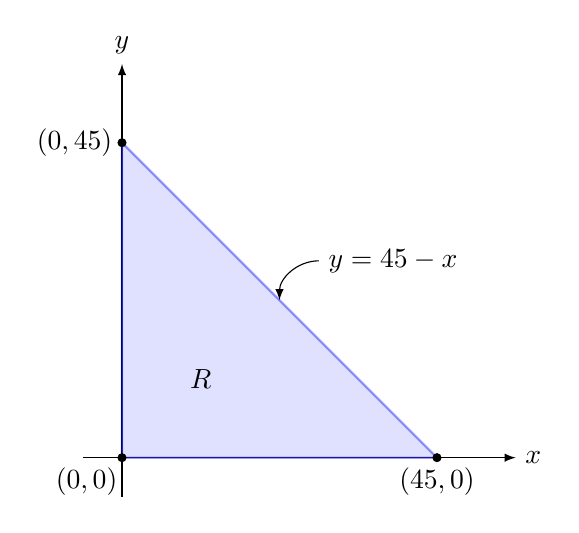
\begin{tikzpicture}
    \draw[-latex] (-0.5, 0) -- (5, 0) node[right] {$x$};
    \draw[-latex] (0, -0.5) -- (0, 5) node[above] {$y$};
    \draw[blue, thick, fill = blue!30, opacity = 0.4] (0,0) -- (0, 4) -- (4, 0)
     -- cycle;
    \draw[fill = black] (0,0) circle (0.05cm) node[below, xshift = -0.45cm] {
    $(0,0)$};
    \draw[fill = black] (4, 0) circle (0.05cm) node[below] {$(45, 0)$};
    \draw[fill = black] (0, 4) circle (0.05cm) node[left] {$(0, 45)$};
    \draw[latex-] (2, 2) arc [start angle = 180, end angle = 90, x radius = 
    0.5cm, y radius = 0.5cm] node[right] {$y = 45 - x$};
    \node[] at (1, 1) {$R$};
\end{tikzpicture}  
\end{center}

We can see that $R = \{(x, y)\text{ }|\text{ }0 \leq x \leq 45,\text{ }0 \leq 
y \leq 45 - x$. Therefore, the probability that Sally's total wait time is less
than 45 minutes is given by:
$$P(X + Y < 45) = \frac{1}{1350} \int_0^{45} \int_0^{45 - x} e^{-x/45} e^{-y/30
}\,dy\,dx$$
$$= \frac{-30}{1350} \int_0^{45} \left(e^{-x/45} \right) \left[e^{-y/30} 
\right]_{y = 0}^{y = 45 - x}\,dx$$
$$= -\frac{1}{45} \int_0^{45} \left( e^{-x/45} \right) \left[ e^{(x - 45)/30} 
- 1 \right]\,dx$$
$$= -\frac{1}{45} \int_0^{45} e^{(x - 135)/90} - e^{-x/45}\,dx$$
$$= -\frac{1}{45} \left[ 90e^{(x - 135)/90} + 45e^{-x/45} \right]_{x = 0}^{x = 
45}$$
$$= - \frac{1}{45} \left[ 90 \left( e^{(45 - 135)/90} - e^{(0 - 135)/90} 
\right) + 45 \left(e^{-45/45} - e^{-0/45} \right) \right]$$
$$= -\frac{1}{45} \left[90 \left( e^{-1} - e^{-3/2} \right) + 45 \left(e^{-1} 
- 1 \right) \right]$$
$$= -\frac{1}{45} \left[135e^{-1} - 90e^{-3/2} - 45 \right] = 1 + 2e^{-3/2} - 
3e^{-1} \approx 0.343$$

So, there is an approximately $34.3\%$ chance Sally will wait less than 45 
minutes to ride both roller coasters. 

\begin{Exercise}[title = {Snow Days}, label = snow]
In order for it to snow, two conditions must be met: the temperature must be 
low enough and the humidity must be high enough. The probability function for 
the temperature, $T$, in Celsius on a winter day is given by:
$$f_1(t) = 
\begin{cases}
    \frac{1}{80} \left[ \cos{\left( \frac{\pi t}{40} \right)} + 1 \right],& 
    -40 \leq t \leq 40\\
    0,&\text{otherwise}
\end{cases}
$$

And the probability function for the humidity, $H$, in percent on the same 
winter day is:
$$f_2(h) = 
\begin{cases}
    \frac{100h - h^2}{500,000},& 0 \leq h \leq 100\\
    0,&\text{otherwise}
\end{cases}
$$

If the temperature must be below freezing and the humidity above 75\% for snow 
to form, what is the probability it snows?
\end{Exercise}

\begin{Answer}[ref = snow]
The joint density function for temperature and humidity is:
$$f(t, h) = f_1(t)f_2(h) = \begin{cases}
    \frac{100h - h^2}{400,000,000}\left[ \cos{\left( \frac{\pi t}{40} \right)} 
    + 1 \right],& 0 \leq h \leq 100\text{, } -40 \leq t \leq 40\\
    0,&\text{otherwise}
\end{cases}$$

And the probability that snow forms is given by:
$$P(T \leq 0, 75 \leq H \leq 100) = \int_{-40}^{0} \int_{75}^{100} \frac{100h 
- h^2}{400,000,000}\left[ \cos{\left( \frac{\pi t}{40} \right)} + 1 \right]\,dh
\,dt$$
$$= \int_{-40}^0 \left(\frac{\cos{ \left( \frac{\pi t}{40} \right)} + 1}{
400,000,000} \right) \int_{75}^{100} \left(100h - h^2 \right)\,dh\,dt$$
$$= \int_{-40}^0 \left(\frac{\cos{ \left( \frac{\pi t}{40} \right)} + 1}{
400,000,000} \right) \left[ 50h^2 - \frac{h^3}{3} \right]_{h = 75}^{h = 100} 
\,dt= \int_{-40}^0 \left(\frac{\cos{ \left( \frac{\pi t}{40} \right)} + 1}{
400,000,000} \right) \left( \frac{78125}{3} \right)\,dt$$
$$= \frac{1}{15360} \int_{-40}^0 \left[ \cos{ \left( \frac{\pi t}{40} \right)} 
+ 1 \right]\,dt = \frac{1}{15360} \left[ \left( \frac{40}{\pi} \right) \sin{ 
\left( \frac{\pi t}{40} \right)} + t \right]_{t = -40}^{t = 0}$$
$$= \frac{1}{15360} (40) = \frac{1}{384} \approx 0.0026$$

So there is a 0.26\% chance it will snow. 
\end{Answer}

\section{Expected Values for Two Variables}
Recall that for one variable, $X$, the expected value of $X$ (its mean) is:
$$\mu = \int_{- \infty}^{\infty} xf(x)\,dx$$

Where $f(x)$ is the probability density function for $X$. Expanding this to two
independent random variables, $X$ and $Y$, we find the expected values for each
variable are:
$$\mu_x = \iint_{\mathbb{R}^2} xf(x, y)\,dA$$
$$\mu_y = \iint_{\mathbb{R}^2} yf(x, y)\,dA$$

\textbf{Example}: $X$ and $Y$ are random variables with joint density function:
$$f(x, y) = 
\begin{cases}
0.1e^{-(0.2x + 0.5y)},&\text{if } x \geq 0,\text{ }y \geq 0\\
0,&\text{otherwise}
\end{cases}$$

What are the expected values of $X$ and $Y$?

\textbf{Solution}: The expected value of $X$ is:
$$\mu_x = \int_0^{\infty} \int_0^{\infty} x(0.1)e^{-(0.2x + 0.5y)}\,dy\,dx$$
$$= \frac{1}{10} \int_0^{\infty} x \left(-2 \right) e^{-(0.2x + 0.5y)}|_{y = 0}
^{y = \infty}\,dx = -\frac{1}{5} \int_0^{\infty} (x)e^{-0.2x} \left[ e^{-0.5y} 
\right]_{y = 0}^{y = \infty}\,dx$$
$$= -\frac{1}{5} \int_0^{\infty} xe^{-0.2x} \left[ e^{-\infty} - e^0 \right]
\,dx = -\frac{1}{5} \int_0^{\infty} xe^{-0.2x} \left[0 - 1 \right]\,dx $$
$$= \frac{1}{5} \int_0^{\infty} xe^{-0.2x}\,dx$$

Applying integration by parts, 
$$\mu_x = \frac{1}{5} \left[ -5xe^{-0.2x}|_{x = 0}^{x = \infty} - \int_0^{
\infty} (-5)e^{-0.2x}\,dx \right]$$
$$= \left[-xe^{-0.2x} \right]_{x = 0}^{x = \infty} + \int_0^{\infty} e^{-0.2x}
\,dx  = -5e^{-0.2x}|_{x = 0}^{x = \infty}$$
$$= -5 \left(e^{-\infty} - e^0 \right) = -5 \left(0 - 1 \right) = 5$$

And the expected value of $Y$ is:
$$\mu_y = \int_0^{\infty} \int_0^{\infty} y(0.1)e^{-(0.2x + 0.5y)}\,dx\,dy$$
$$= \frac{1}{10} \int_0^{\infty} (y)e^{-0.5y} \int_0^{\infty} \left(e^{-0.2x} 
\right)\,dx\,dy = \frac{1}{10} \int_0^{\infty} (y)e^{-0.5y} \left[ -5e^{-0.2x} 
\right]_{x = 0}^{x = \infty}\,dy$$
$$= \frac{1}{10} \int_0^{\infty} (y)e^{-0.5y} \left(0 + 5 \right)\,dy = \frac{
1}{2} \int_0^{\infty} ye^{-0.5y}\,dy$$

Applying integration by parts:
$$\mu_y = \frac{1}{2} \left[(-2)ye^{-0.5y}|_{y = 0}^{y = \infty} - \int_0^{
\infty} (-2)e^{-0.5y}\,dy \right]$$
$$= \left[-ye^{-0.5y} \right]_{y = 0}^{y = \infty} + (-2)e^{-0.5y}|_{y = 0}^{y 
= \infty} = (-2) \left( e^{-infty} - e^0 \right) = -2(0 - 1) = 2$$

Therefore, the expected value of $X$ is 5 and of $Y$ is 2. 

\begin{Exercise}[title = {Expected Values}, label = expect]
The joint density function for a pair of random variables, $X$ and $Y$ is
$$f(x, y) = 
\begin{cases}
	\frac{1}{4} y (1 + 2x),& \text{if } 0 \leq x \leq 1\text{, }0 \leq y \leq 2\\
	0,&\text{ otherwise}
\end{cases}$$
What are the expected values of $X$ and $Y$?
\end{Exercise}

\begin{Answer}[ref = expect]
Finding the expected value of $X$:
$$\mu_x = \int_0^1 \int_0^2 \frac{1}{4}xy \left(1 + 2x \right)\,dy\,dx = 
\frac{1}{4} \int_0^1 x \left( 1 + 2x \right) \int_0^2 y\,dy\,dx$$
$$= \frac{1}{4} \int_0^1 x \left( 1 + 2x \right) \left[ \frac{1}{2} y^2 \right]_
{y = 0}^{y = 2}\,dx = \frac{1}{4} \int_0^1 x \left(1 + 2x \right) (2)\,dx$$
$$= \frac{1}{2} \int_0^1 x + 2x^2\,dx = \frac{1}{2} \left[ \frac{1}{2}x^2 + 
\frac{2}{3}x^3 \right]_{x = 0}^{x = 1}$$
$$= \frac{1}{2} \left( \frac{1}{2} + \frac{2}{3} \right) = \frac{1}{2} \left( 
\frac{7}{6} \right) = \frac{7}{12}$$

And finding the expected value of $Y$:
$$\mu_y = \int_0^2 \int_0^1 \frac{1}{4}y^2 \left(1 + 2x \right)\,dx\,dy = 
\frac{1}{4} \int_0^2 y^2 \int_0^1 \left( 1 + 2x \right)\,dx\,dy$$
$$= \frac{1}{4} \int_0^2 y^2 \left[x + x^2 \right]_{x = 0}^{x = 1}\,dy = 
\frac{1}{4} \int_0^2 y^2 (2)\,dy$$
$$= \frac{1}{2} \int_0^2 y^2\,dy = \frac{1}{2} \left[ \frac{1}{3}y^3 \right]_{
y = 0}^{y = 2} = \frac{1}{2} \left( \frac{1}{3} \right) (8) = \frac{4}{3}$$
\end{Answer}